% ------------------------------------------------------------------------------------------------------------------
% Basic configuration and packages
% ------------------------------------------------------------------------------------------------------------------
% Package for discovering wrong and outdated usage of LaTeX.
% More information to be found in l2tabu English version.
\RequirePackage[l2tabu, orthodox]{nag}
% Class of LaTeX document: {size of paper, size of font}[document class]
\documentclass[a4paper,11pt]{article}



% ------------------------------------------------------
% Packages not tied to particular normal language
% ------------------------------------------------------
% This package should improved spaces in the text
\usepackage{microtype}
% Add few important symbols, like text Celcius degree
\usepackage{textcomp}



% ------------------------------------------------------
% Polonization of LaTeX document
% ------------------------------------------------------
% Basic polonization of the text
\usepackage[MeX]{polski}
% Switching on UTF-8 encoding
\usepackage[utf8]{inputenc}
% Adding font Latin Modern
\usepackage{lmodern}
% Package is need for fonts Latin Modern
\usepackage[T1]{fontenc}



% ------------------------------------------------------
% Setting margins
% ------------------------------------------------------
\usepackage[a4paper, total={14cm, 25cm}]{geometry}



% ------------------------------------------------------
% Setting vertical spaces in the text
% ------------------------------------------------------
% Setting space between lines
\renewcommand{\baselinestretch}{1.1}

% Setting space between lines in tables
\renewcommand{\arraystretch}{1.4}



% ------------------------------------------------------
% Packages for scientific papers
% ------------------------------------------------------
% Switching off \lll symbol, that I guess is representing letter "Ł"
% It collide with `amsmath' package's command with the same name
\let\lll\undefined
% Basic package from American Mathematical Society (AMS)
\usepackage[intlimits]{amsmath}
% Equations are numbered separately in every section
\numberwithin{equation}{section}

% Other very useful packages from AMS
\usepackage{amsfonts}
\usepackage{amssymb}
\usepackage{amscd}
\usepackage{amsthm}

% Package with better looking calligraphy fonts
\usepackage{calrsfs}

% Package with better looking greek letters
% Example of use: pi -> \uppi
\usepackage{upgreek}
% Improving look of lambda letter
\let\oldlambda\lambda
\renewcommand{\lambda}{\uplambda}




% ------------------------------------------------------
% BibLaTeX
% ------------------------------------------------------
% Package biblatex, with biber as its backend, allow us to handle
% bibliography entries that use Unicode symbols outside ASCII
% \usepackage[
% language=polish,
% backend=biber,
% style=alphabetic,
% url=false,
% eprint=true,
% ]{biblatex}

% \addbibresource{Logika-i-teoria-mnogości-Bibliography.bib}





% ------------------------------------------------------
% Defining new environments (?)
% ------------------------------------------------------
% Defining enviroment "Wniosek"
% \newtheorem{corollary}{Wniosek}
% \newtheorem{definition}{Definicja}
% \newtheorem{theorem}{Twierdzenie}





% ------------------------------------------------------
% Wonderful package PGF/TikZ
% ------------------------------------------------------
\usepackage{tikz}

\usepackage[dvipsnames]{xcolor}

% Loding TikZ libraries

% % Library for positioning nodes
% \usetikzlibrary{positioning}

% % Styles for arrows
% \usepackage{./Local-packages/PGF-TikZ-Arrows-styles}

% % Node and pics for drawing charts
% \usepackage{./Local-packages/PGF-TikZ-Chart-nodes-and-pics}




% ------------------------------------------------------
% Local packages
% ------------------------------------------------------
% Local configuration of this particular file
\usepackage{./Local-packages/local-settings}

% Package containing various command useful for working with a text
% \usepackage{general-commands}
% Package containing commands and other code useful for working with
% mathematical text
% \usepackage{math-commands}





% ------------------------------------------------------
% Package "hyperref"
% They advised to put it on the end of preambule
% ------------------------------------------------------
% It allows you to use hyperlinks in the text
\usepackage{hyperref}










% ------------------------------------------------------------------------------------------------------------------
% Title and author of the text
\title{Kolory z~paczki \texttt{xcolor}}

\author{Kamil Ziemian \\
  \email}


% \date{}
% ------------------------------------------------------------------------------------------------------------------










% ####################################################################
% Beginning of the document
\begin{document}
% ####################################################################





% ######################################
% Title of the text
\maketitle
% ######################################





% % ######################################
% \section{Gładkie funkcje o~zwartym nośniku}

% \label{sec:Funkcje-wykladnicze-i-logarytmiczne}
% % ######################################



% ##################
\begin{figure}

  \label{fig:Smooth-function-with-compact-support-01}


  \centering

  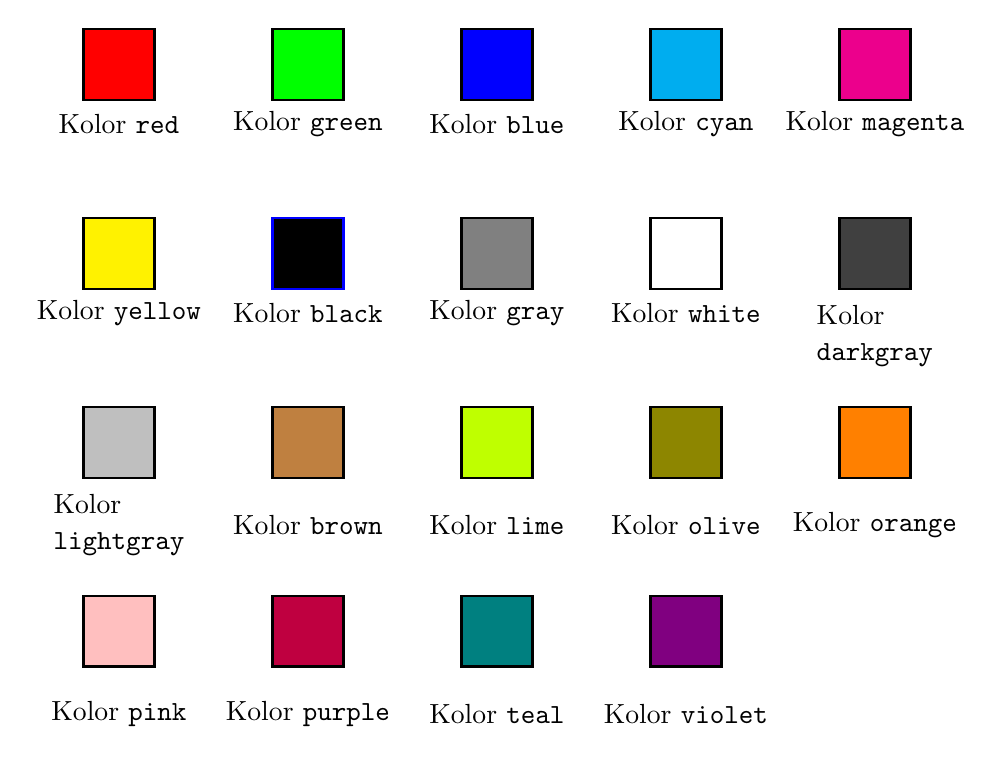
\begin{tikzpicture}[scale=3]

    \filldraw[draw=black,line width=1,fill=red] (0,0) rectangle (0.3,0.3);

    \node at (0.15,-0.1) {Kolor \texttt{red}};



    \begin{scope}[xshift=0.8cm]

      \filldraw[draw=black,line width=1,fill=green]
      (0,0) rectangle (0.3,0.3);

      \node at (0.15,-0.1) {Kolor \texttt{green}};

    \end{scope}



    \begin{scope}[xshift=1.6cm]

      \filldraw[draw=black,line width=1,fill=blue]
      (0,0) rectangle (0.3,0.3);

      \node at (0.15,-0.1) {Kolor \texttt{blue}};

    \end{scope}



    \begin{scope}[xshift=2.4cm]

      \filldraw[draw=black,line width=1,fill=cyan]
      (0,0) rectangle (0.3,0.3);

      \node at (0.15,-0.1) {Kolor \texttt{cyan}};

    \end{scope}



    \begin{scope}[xshift=3.2cm]

      \filldraw[draw=black,line width=1,fill=magenta]
      (0,0) rectangle (0.3,0.3);

      \node at (0.15,-0.1) {Kolor \texttt{magenta}};

    \end{scope}





    \begin{scope}[yshift=-0.8cm]

      \filldraw[draw=black,line width=1,fill=yellow]
      (0,0) rectangle (0.3,0.3);

      \node at (0.15,-0.1) {Kolor \texttt{yellow}};

    \end{scope}



    \begin{scope}[xshift=0.8cm,yshift=-0.8cm]

      \filldraw[draw=blue,line width=1,fill=black]
      (0,0) rectangle (0.3,0.3);

      \node at (0.15,-0.1) {Kolor \texttt{black}};

    \end{scope}



    \begin{scope}[xshift=1.6cm,yshift=-0.8cm]

      \filldraw[draw=black,line width=1,fill=gray]
      (0,0) rectangle (0.3,0.3);

      \node at (0.15,-0.1) {Kolor \texttt{gray}};

    \end{scope}



    \begin{scope}[xshift=2.4cm,yshift=-0.8cm]

      \filldraw[draw=black,line width=1,fill=white]
      (0,0) rectangle (0.3,0.3);

      \node at (0.15,-0.1) {Kolor \texttt{white}};

    \end{scope}



    \begin{scope}[xshift=3.2cm,yshift=-0.8cm]

      \filldraw[draw=black,line width=1,fill=darkgray]
      (0,0) rectangle (0.3,0.3);

      \node[align=left] at (0.15,-0.2)
      {Kolor \\
        \texttt{darkgray}};

    \end{scope}



    \begin{scope}[yshift=-1.6cm]

      \filldraw[draw=black,line width=1,fill=lightgray]
      (0,0) rectangle (0.3,0.3);

      \node[align=left] at (0.15,-0.2)
      {Kolor \\
        \texttt{lightgray}};

    \end{scope}



    \begin{scope}[xshift=0.8cm,yshift=-1.6cm]

      \filldraw[draw=black,line width=1,fill=brown]
      (0,0) rectangle (0.3,0.3);

      \node at (0.15,-0.2) {Kolor \texttt{brown}};

    \end{scope}



    \begin{scope}[xshift=1.6cm,yshift=-1.6cm]

      \filldraw[draw=black,line width=1,fill=lime]
      (0,0) rectangle (0.3,0.3);

      \node at (0.15,-0.2) {Kolor \texttt{lime}};

    \end{scope}



    \begin{scope}[xshift=2.4cm,yshift=-1.6cm]

      \filldraw[draw=black,line width=1,fill=olive]
      (0,0) rectangle (0.3,0.3);

      \node at (0.15,-0.2) {Kolor \texttt{olive}};

    \end{scope}



    \begin{scope}[xshift=3.2cm,yshift=-1.6cm]

      \filldraw[draw=black,line width=1,fill=orange]
      (0,0) rectangle (0.3,0.3);

      \node at (0.15,-0.2) {Kolor \texttt{orange}};

    \end{scope}





    \begin{scope}[yshift=-2.4cm]

      \filldraw[draw=black,line width=1,fill=pink]
      (0,0) rectangle (0.3,0.3);

      \node at (0.15,-0.2) {Kolor \texttt{pink}};

    \end{scope}



    \begin{scope}[xshift=0.8cm,yshift=-2.4cm]

      \filldraw[draw=black,line width=1,fill=purple]
      (0,0) rectangle (0.3,0.3);

      \node at (0.15,-0.2) {Kolor \texttt{purple}};

    \end{scope}



    \begin{scope}[xshift=1.6cm,yshift=-2.4cm]

      \filldraw[draw=black,line width=1,fill=teal]
      (0,0) rectangle (0.3,0.3);

      \node at (0.15,-0.2) {Kolor \texttt{teal}};

    \end{scope}



    \begin{scope}[xshift=2.4cm,yshift=-2.4cm]

      \filldraw[draw=black,line width=1,fill=violet]
      (0,0) rectangle (0.3,0.3);

      \node at (0.15,-0.2) {Kolor \texttt{violet}};

    \end{scope}

  \end{tikzpicture}

  \caption{Kolor bazowe paczki
    \href{https://ctan.org/pkg/xcolor}{\texttt{xcolor}}}


\end{figure}
% ##################





% ##################
\begin{figure}

  \label{fig:Smooth-function-with-compact-support-01}


  \centering

  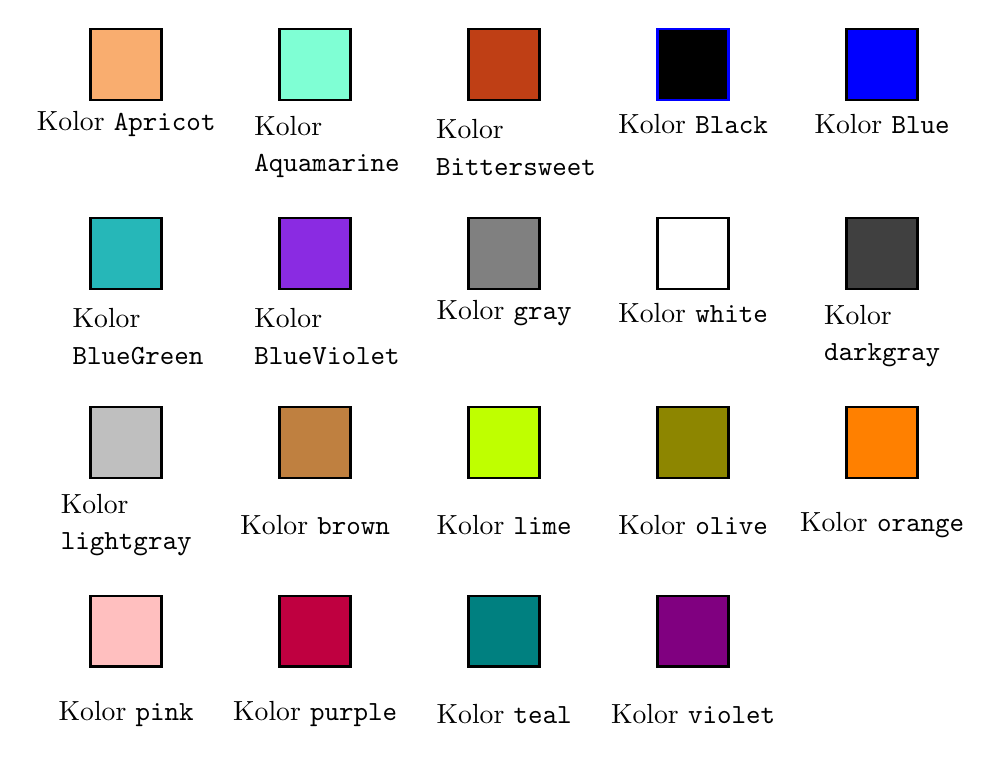
\begin{tikzpicture}[scale=3]

    \filldraw[draw=black,line width=1,fill=Apricot]
    (0,0) rectangle (0.3,0.3);

    \node at (0.15,-0.1) {Kolor \texttt{Apricot}};



    \begin{scope}[xshift=0.8cm]

      \filldraw[draw=black,line width=1,fill=Aquamarine]
      (0,0) rectangle (0.3,0.3);

      \node[align=left] at (0.2,-0.2)
      {Kolor \\
        \texttt{Aquamarine}};

    \end{scope}



    \begin{scope}[xshift=1.6cm]

      \filldraw[draw=black,line width=1,fill=Bittersweet]
      (0,0) rectangle (0.3,0.3);

      \node[align=left] at (0.2,-0.2)
      {Kolor \\
        \texttt{Bittersweet}};

    \end{scope}



    \begin{scope}[xshift=2.4cm]

      \filldraw[draw=blue,line width=1,fill=Black]
      (0,0) rectangle (0.3,0.3);

      \node at (0.15,-0.1) {Kolor \texttt{Black}};

    \end{scope}



    \begin{scope}[xshift=3.2cm]

      \filldraw[draw=black,line width=1,fill=Blue]
      (0,0) rectangle (0.3,0.3);

      \node at (0.15,-0.1) {Kolor \texttt{Blue}};

    \end{scope}





    \begin{scope}[yshift=-0.8cm]

      \filldraw[draw=black,line width=1,fill=BlueGreen]
      (0,0) rectangle (0.3,0.3);

      \node[align=left] at (0.2,-0.2)
      {Kolor \\
        \texttt{BlueGreen}};

    \end{scope}



    \begin{scope}[xshift=0.8cm,yshift=-0.8cm]

      \filldraw[draw=black,line width=1,fill=BlueViolet]
      (0,0) rectangle (0.3,0.3);

      \node[align=left] at (0.2,-0.2)
      {Kolor \\
        \texttt{BlueViolet}};

    \end{scope}



    \begin{scope}[xshift=1.6cm,yshift=-0.8cm]

      \filldraw[draw=black,line width=1,fill=gray]
      (0,0) rectangle (0.3,0.3);

      \node at (0.15,-0.1) {Kolor \texttt{gray}};

    \end{scope}



    \begin{scope}[xshift=2.4cm,yshift=-0.8cm]

      \filldraw[draw=black,line width=1,fill=white]
      (0,0) rectangle (0.3,0.3);

      \node at (0.15,-0.1) {Kolor \texttt{white}};

    \end{scope}



    \begin{scope}[xshift=3.2cm,yshift=-0.8cm]

      \filldraw[draw=black,line width=1,fill=darkgray]
      (0,0) rectangle (0.3,0.3);

      \node[align=left] at (0.15,-0.2)
      {Kolor \\
        \texttt{darkgray}};

    \end{scope}



    \begin{scope}[yshift=-1.6cm]

      \filldraw[draw=black,line width=1,fill=lightgray]
      (0,0) rectangle (0.3,0.3);

      \node[align=left] at (0.15,-0.2)
      {Kolor \\
        \texttt{lightgray}};

    \end{scope}



    \begin{scope}[xshift=0.8cm,yshift=-1.6cm]

      \filldraw[draw=black,line width=1,fill=brown]
      (0,0) rectangle (0.3,0.3);

      \node at (0.15,-0.2) {Kolor \texttt{brown}};

    \end{scope}



    \begin{scope}[xshift=1.6cm,yshift=-1.6cm]

      \filldraw[draw=black,line width=1,fill=lime]
      (0,0) rectangle (0.3,0.3);

      \node at (0.15,-0.2) {Kolor \texttt{lime}};

    \end{scope}



    \begin{scope}[xshift=2.4cm,yshift=-1.6cm]

      \filldraw[draw=black,line width=1,fill=olive]
      (0,0) rectangle (0.3,0.3);

      \node at (0.15,-0.2) {Kolor \texttt{olive}};

    \end{scope}



    \begin{scope}[xshift=3.2cm,yshift=-1.6cm]

      \filldraw[draw=black,line width=1,fill=orange]
      (0,0) rectangle (0.3,0.3);

      \node at (0.15,-0.2) {Kolor \texttt{orange}};

    \end{scope}





    \begin{scope}[yshift=-2.4cm]

      \filldraw[draw=black,line width=1,fill=pink]
      (0,0) rectangle (0.3,0.3);

      \node at (0.15,-0.2) {Kolor \texttt{pink}};

    \end{scope}



    \begin{scope}[xshift=0.8cm,yshift=-2.4cm]

      \filldraw[draw=black,line width=1,fill=purple]
      (0,0) rectangle (0.3,0.3);

      \node at (0.15,-0.2) {Kolor \texttt{purple}};

    \end{scope}



    \begin{scope}[xshift=1.6cm,yshift=-2.4cm]

      \filldraw[draw=black,line width=1,fill=teal]
      (0,0) rectangle (0.3,0.3);

      \node at (0.15,-0.2) {Kolor \texttt{teal}};

    \end{scope}



    \begin{scope}[xshift=2.4cm,yshift=-2.4cm]

      \filldraw[draw=black,line width=1,fill=violet]
      (0,0) rectangle (0.3,0.3);

      \node at (0.15,-0.2) {Kolor \texttt{violet}};

    \end{scope}

  \end{tikzpicture}

  \caption{Kolor z~grupy \texttt{dvipsnames} z~paczki
    \href{https://ctan.org/pkg/xcolor}{\texttt{xcolor}}}


\end{figure}
% ##################










% % ######################################
% \section{Funkcje trygonometryczne}

% \label{sec:Funkcje-trygonometryczne}
% % ######################################

















% ####################################################################
% ####################################################################
% Bibliography

% \printbibliography





% ############################
% End of the document

\end{document}
